\section{The Explanation Layer: Standards-Grounded Criticality Attribution}
\label{sec:5}

A ranking says where risk is highest, not how to reduce it. A component may be critical because it is an unreplicated single point of failure, an error-propagating cascade hub, or a high-coupling maintainability bottleneck. Each of these calls for a different intervention: replication, circuit breakers, or decoupling. The explanation layer attributes these causes after ranking. It reads the same node properties (Section~\ref{sec:3.4}), shares no parameters with the engines, and is not used as a ranker. We present it as a design proposal: its attributions are traceable to named metrics and standard sub-characteristics, but they have not yet been validated against developer judgement or against the outcome of the repairs they recommend (Section~\ref{sec:limitations}).

\subsection{Grounding in ISO/IEC Standards}
\label{sec:5.1}

Following ISO/IEC 25010:2023 \cite{iso25010_2023} and ISO/IEC 25019:2023 \cite{iso25019_2023}, criticality is profiled along \textbf{Reliability ($R$)}, split into \textbf{Fault Tolerance ($FT$)} and \textbf{Availability ($A$)}, and \textbf{Maintainability ($M$)}. $FT$ captures error-cascade potential and informs circuit breakers and redundancy. $A$ captures structural single points of failure and informs replication. $M$ captures coupling and code-level complexity and informs decoupling and refactoring. Safety and security, which need hazard logs, are out of scope.

\subsection{Composite Quality Score}
\label{sec:5.2}

Figure~\ref{fig:rm} summarizes the layer. All metrics are rank-normalized to $[0, 1]$ within the graph and combined with AHP-derived weights \cite{saaty1980ahp}:
\begin{itemize}\tightlist
    \item $FT(v) = 0.45 \cdot \text{RPR}(v) + 0.30 \cdot \text{Deg}_{\text{in}}(v) + 0.25 \cdot \text{CDPot}_{\text{enh}}(v)$, over Reverse PageRank, normalized in-degree and normalized cascade depth on $G_{\text{analysis}}^\top$;
    \item $A(v) = 0.25 \cdot \text{AP}_c^{\text{dir}}(v) + 0.20 \cdot \text{QSPOF}(v) + 0.20 \cdot \text{BR}(v) + 0.25 \cdot \text{CDI}(v) + 0.10 \cdot w(v)$, over directed articulation severity, QoS-weighted SPOF severity, bridge ratio, the Connectivity Degradation Index and the node QoS weight;
    \item $R(v) = r_{\text{FT}} \cdot FT(v) + (1 - r_{\text{FT}}) \cdot A(v)$ with $r_{\text{FT}} = 0.36$;
    \item $M(v) = 0.35 \cdot \text{BT}(v) + 0.30 \cdot w_{\text{out}}(v) + 0.15 \cdot \text{CQP}(v) + 0.12 \cdot \text{CouplingRisk}_{\text{enh}}(v) + 0.08 \cdot (1 - \text{CC}(v))$, over betweenness, QoS-weighted efferent coupling, code-quality penalty, coupling risk and clustering.
\end{itemize}
The composite is $Q(v) = 0.80 \cdot R(v) + 0.20 \cdot M(v)$, and an ISO/IEC 25019 context-of-use vector can reweight $R$ and $M$. Intra-dimension weights are shrunk towards a uniform prior ($\lambda = 0.70$). The elicited weights are not predictive: used as a ranker, $Q(v)$ scores $\rho = 0.205$ against $I^*$ under LOSO, below every centrality baseline, and moving from the elicited towards a uniform prior improves it ($0.200 \to 0.319$; Supplementary Sections~\ref{S-supp:params} and~\ref{S-supp:loso-active}). $Q(v)$ is therefore used only to name the dimension along which a flagged component is weak, never to decide which components are flagged. The AHP matrices and their consistency diagnostics are in Supplementary Section~\ref{S-supp:ahp}. Within the explanation layer, components above the Tukey upper fence of $Q$ are marked CRITICAL (mean $4.2\%$ of components); in the pipeline, the components profiled are the ranking's top-$K$. High $A$ with low $FT$ indicates a single point of failure that needs replication, while high $FT$ indicates a cascade hub that needs circuit breakers (example card: Supplementary Section~\ref{S-supp:card}).

\begin{figure}[htbp]
\centering
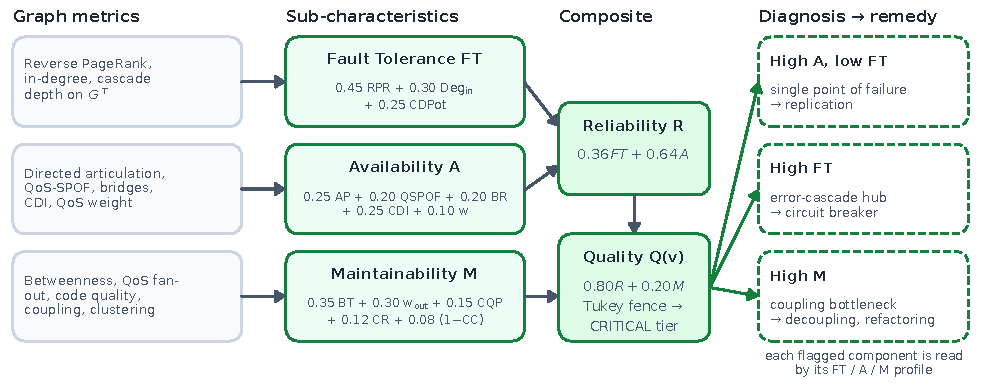
\includegraphics[width=\linewidth]{figures/Figure_4}
\caption{The explanation layer. Rank-normalized graph metrics feed the ISO/IEC 25010 sub-characteristics Fault Tolerance, Availability and Maintainability (CR: coupling risk; CC: clustering coefficient), which combine into Reliability and the composite $Q(v)$. A component above the Tukey fence of $Q$ is flagged, and its $FT$/$A$/$M$ profile names the remediation class.}
\label{fig:rm}
\end{figure}

\subsection{Counterfactual Verification of Remediation}
\label{sec:5.3}

The replication package includes tooling that generates candidate repairs (broker replication, circuit-breaker insertion, topic decoupling) for flagged components and verifies them counterfactually in memory: a repair is accepted only if it reduces systemic impact beyond seed noise ($\Delta \bar{I}_{\text{comp}} > \kappa \cdot \sigma_{\text{seed}}$, $\kappa \ge 1$) without introducing new articulation points. This paper reports no result from it. Comparing the repair class the layer recommends against alternative repairs under this verifier is the most direct test of the attributions, and is future work together with a developer study.
